\documentclass[11pt]{article}

\usepackage[margin=1in]{geometry}
\usepackage[T1]{fontenc}
\usepackage{lmodern}
\usepackage{microtype}
\usepackage{amsmath, amssymb}
\usepackage{booktabs}
\usepackage{array}
\usepackage{tabularx}
\usepackage{tikz}
\usetikzlibrary{arrows.meta, positioning, shapes.geometric, calc, decorations.pathreplacing, backgrounds}
\usepackage{float}
\usepackage[hidelinks]{hyperref}
\usepackage{caption}
\usepackage{xcolor}
\usepackage{enumitem}
\usepackage[round]{natbib}

\setlength{\parskip}{0.5em}
\setlength{\parindent}{0pt}

\newcommand{\predstart}{\text{pred\_start}}
\newcommand{\predstop}{\text{pred\_stop}}
\newcommand{\scr}{\text{SCr}}
\newcommand{\tkdtwo}{t_{\text{KDIGO2}}}

\title{\textbf{FLAIR Task Schematic} \\[0.3em]
       AKI KDIGO Stage 2 within 24 Hours (Task T5)}
\author{FLAIR Benchmark}
\date{\today}

\begin{document}
\maketitle

\begin{abstract}
\noindent We specify the FLAIR continuous AKI task: at every hourly
decision point during the first ICU stay, predict whether the patient
will meet the KDIGO stage 2 serum-creatinine criterion within the next
24 hours. The label, baseline rule, and cohort exclusions follow
\citet{koyner2018aki}; urine-output criteria are not used. One cohort
deviation (KDIGO/Koyner exclusion rule 2 --- ICD CKD stage 4+) is
documented because CLIF \texttt{Diagnoses} is not yet exposed via the
FLAIR loaders.
\end{abstract}

\section{FLAIR operational definition}
\label{sec:def}

\subsection{Anchors and windows}

Let $H_i$ denote a hospitalization with first ICU stay window
$[t^{\text{ICU}_1,\text{start}}_i,\, t^{\text{ICU}_1,\text{end}}_i]$
returned by \verb|compute_icu_timing| from the CLIF \texttt{ADT} table.

\begin{description}[leftmargin=2em, style=nextline]

\item[Serum-creatinine baseline.]
For each SCr measurement $\scr_i(t)$ with $t$
$=$ \texttt{lab\_result\_dttm},
\[
\text{baseline}_i(t) \;=\;
\begin{cases}
\min\!\bigl\{\scr_i(\tau)\,:\,\tau \in (t-168\text{h},\,t)\bigr\}
  & \text{if non-empty,}\\[0.4em]
\scr_i\!\bigl(t^{\text{index}}_i\bigr)
  & \text{otherwise (index SCr fallback)}
\end{cases}
\]
where $t^{\text{index}}_i$ is the earliest in-stay SCr of $H_i$. The
window is strictly left-exclusive of $t$ (the current measurement is
\emph{not} part of its own baseline).

\item[KDIGO stage 2 flag.]
$\mathbb{1}_{\text{KDIGO2}}(t) = \mathbb{1}\!\left[\scr_i(t) \,\ge\, 2.0 \cdot
\text{baseline}_i(t)\right]$.

\item[First-onset time.]
$\tkdtwo^i = \min\{\,t \mid \mathbb{1}_{\text{KDIGO2}}(t) = 1\,\}$;
$\tkdtwo^i = +\infty$ if the patient never meets KDIGO-2 during the
first ICU stay.

\item[Prediction-window start ($\predstart$).]
$\predstart_i = t^{\text{ICU}_1,\text{start}}_i$.

\item[Prediction-window stop ($\predstop$).]
$\predstop_i = \min\!\bigl(t^{\text{ICU}_1,\text{end}}_i,\,
\tkdtwo^i\bigr)$. The interval $[\predstart_i, \predstop_i)$ is
closed-open; $\tkdtwo^i$ itself is \emph{not} a decision point.

\item[Decision-point grid.]
Hourly grid:
$D_i = \{\predstart_i + k\!\cdot\!1\text{h} : k\in\mathbb{Z}_{\ge 0},\,
\predstart_i + k\!\cdot\!1\text{h} < \predstop_i\}$.

\item[Label (\texttt{label\_aki\_kdigo2\_24h}).]
For $d \in D_i$:
\[
y_i(d) = \mathbb{1}\!\left[\tkdtwo^i \in (d,\ d + 24\text{h}\,]\right].
\]
Patients who never meet KDIGO-2 ($\tkdtwo^i = +\infty$) contribute
all-negative rows over $[\predstart_i, t^{\text{ICU}_1,\text{end}}_i)$.

\end{description}

\subsection{Cohort (Koyner 2018)}

\begin{itemize}[leftmargin=2em]
  \item Age at admission $\ge 18$ with valid \texttt{admission\_dttm}
        and \texttt{discharge\_dttm}.
  \item $\geq 1$ ICU ADT record (first ICU stay defined).
  \item $\geq 1$ creatinine measurement during the first ICU stay
        (baseline must be computable).
  \item \textbf{Exclude} first SCr $\ge 3.0$ mg/dL (Koyner rule 1;
        implemented).
  \item \textbf{Exclude} RRT within 48h of first SCr (Koyner rule 3;
        implemented when an RRT table is provided, skipped here as the
        RRT loader is not wired).
  \item \textbf{Not applied}: ICD CKD stage 4+ (Koyner rule 2). The
        CLIF \texttt{Diagnoses} table is not yet exposed via
        \texttt{flair\_benchmark/\_clif.py}; this is a documented
        deviation and is flagged in the main-paper Limitations.
\end{itemize}

\subsection{CLIF tables and categories used}
\label{sec:t5-clif}

Task~T5 reads four CLIF v2.1 tables. The cohort entry filter is on
\texttt{adt.location\_category}; the KDIGO-2 signal is computed from a
single category-column filter in \texttt{labs}.

\begin{table}[H]
\centering
\small
\begin{tabular}{@{}llp{7.0cm}@{}}
\toprule
\textbf{CLIF table} & \textbf{Category column} & \textbf{Literal values kept (case-insensitive)} \\
\midrule
\texttt{hospitalization} & ---                       & cohort/demographics join; no category filter \\
\texttt{patient}         & ---                       & demographics join; no category filter \\
\texttt{adt}             & \texttt{location\_category} & $\{\texttt{"icu"}\}$ \\
\texttt{labs}            & \texttt{lab\_category}     & $\{\texttt{"creatinine"}\}$ (loader-side filter) \\
\bottomrule
\end{tabular}
\caption{CLIF surface for Task~T5. The \texttt{labs} filter is applied
inside \texttt{load\_labs(lab\_categories=["creatinine"])} so non-SCr
rows never enter memory.}
\end{table}

Columns selected from each table:
\begin{itemize}[leftmargin=2em, itemsep=0pt]
  \item \texttt{hospitalization}: \texttt{hospitalization\_id},
        \texttt{patient\_id}, \texttt{admission\_dttm},
        \texttt{discharge\_dttm}, \texttt{age\_at\_admission},
        \texttt{discharge\_category}.
  \item \texttt{patient}: \texttt{patient\_id},
        \texttt{sex\_category}, \texttt{race\_category},
        \texttt{ethnicity\_category}, \texttt{death\_dttm}.
  \item \texttt{adt}: \texttt{hospitalization\_id},
        \texttt{location\_category}, \texttt{in\_dttm},
        \texttt{out\_dttm}.
  \item \texttt{labs}: \texttt{hospitalization\_id},
        \texttt{lab\_category}, \texttt{lab\_result\_dttm},
        \texttt{lab\_value\_numeric}.
\end{itemize}

\paragraph{CLIF surfaces specified but not loaded (deviations).}
Two CLIF surfaces appear in the operational definition above but are
not currently exercised by the build pipeline:
\begin{itemize}[leftmargin=2em, itemsep=0pt]
  \item \textbf{CLIF \texttt{patient\_problem\_list} (or Diagnoses).}
        Required to implement Koyner exclusion rule~2 (CKD stage 4+).
        Not exposed by \texttt{flair\_benchmark/\_clif.py}; the rule is
        skipped and the deviation is rendered as a gray-dashed node in
        Figure~\ref{fig:aki-flow}.
  \item \textbf{RRT signal source.} Koyner exclusion rule~3 expects
        an RRT-bearing table (a procedures-style table or
        \texttt{respiratory\_support} with CRRT in
        \texttt{device\_category}). \texttt{apply\_koyner\_exclusions}
        is currently called with \texttt{rrt\_df=None}, so rule~3 is
        not enforced. Adding the loader is mechanical and would not
        change the schematic, only the realized cohort.
\end{itemize}

\section{Algorithmic flow}
\label{sec:flow}

\begin{figure}[H]
\centering
% Algorithmic flowchart for FLAIR AKI KDIGO-2 task build pipeline.

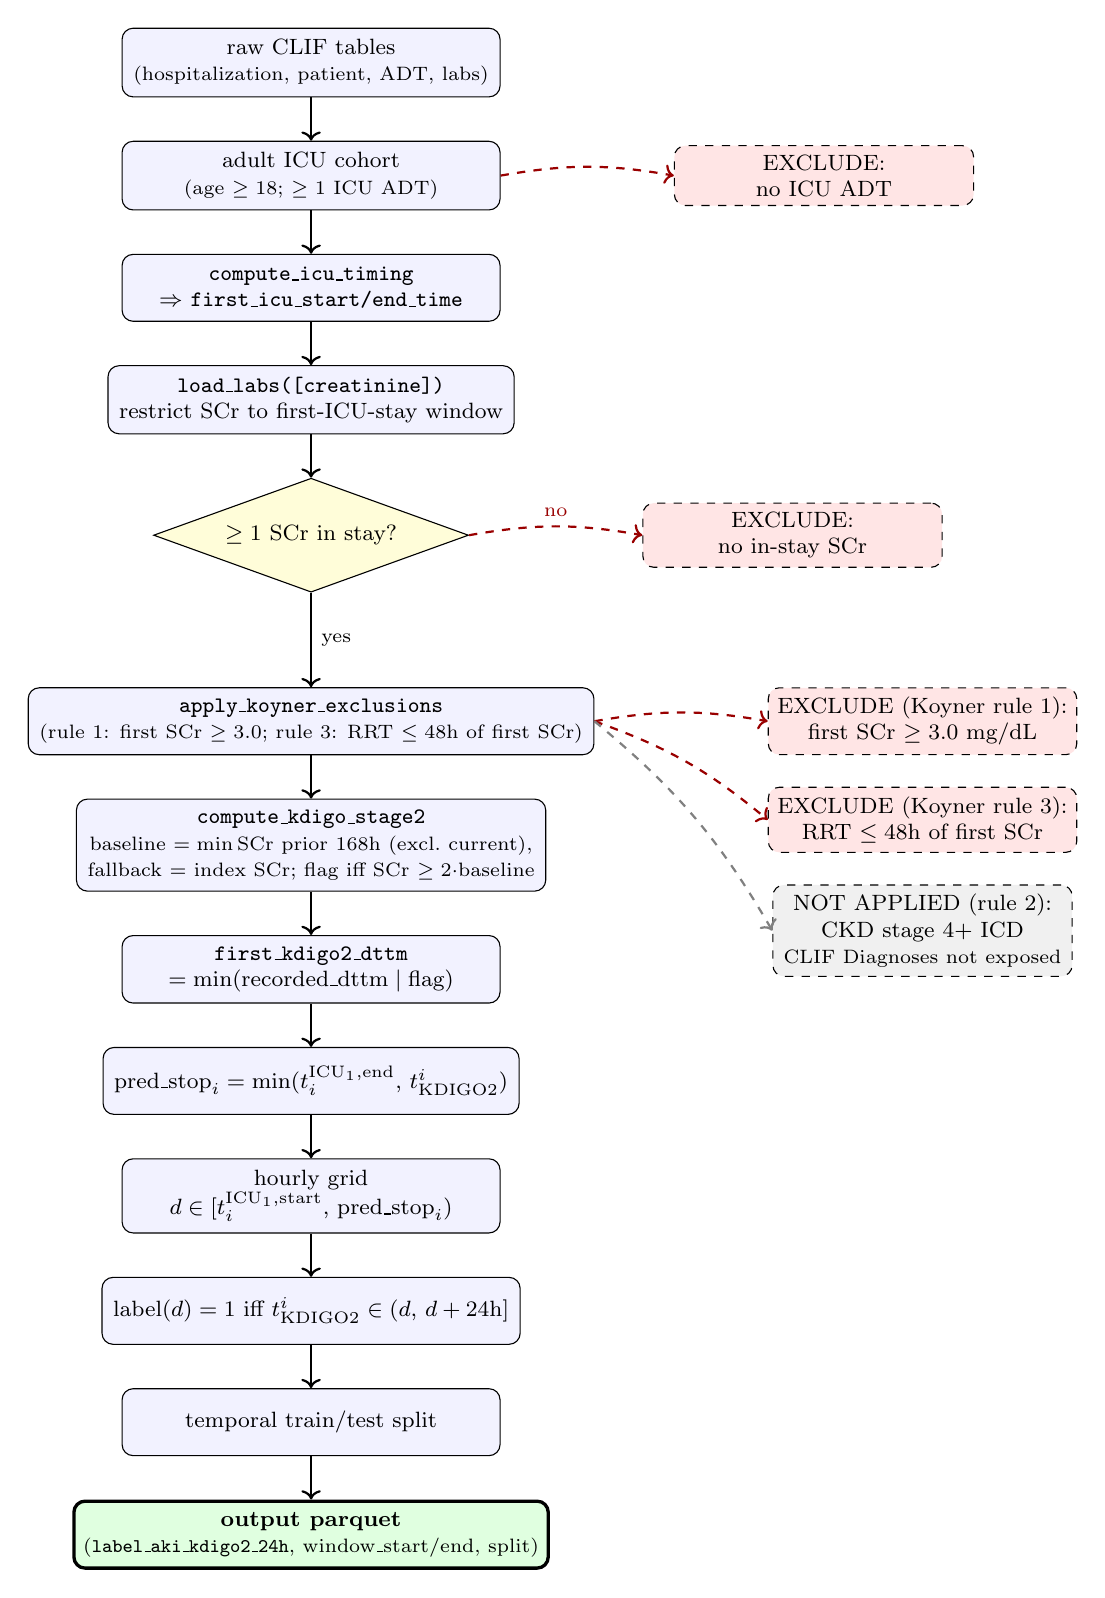
\begin{tikzpicture}[
    node distance=0.55cm and 0.7cm,
    every node/.style={font=\footnotesize, align=center},
    box/.style={draw, rounded corners, fill=blue!5,
                minimum width=4.8cm, minimum height=0.85cm, inner sep=4pt},
    dbox/.style={draw, diamond, aspect=2.2, fill=yellow!15,
                 minimum width=4.0cm, inner sep=2pt},
    excl/.style={draw, rounded corners, fill=red!10, dashed,
                 minimum width=3.8cm, minimum height=0.7cm},
    notapplied/.style={draw, rounded corners, fill=gray!12, dashed,
                       minimum width=3.8cm, minimum height=0.7cm},
    outbox/.style={draw, rounded corners, fill=green!12, very thick,
                minimum width=4.8cm, minimum height=0.85cm},
    arrow/.style={->, thick},
    sidearrow/.style={->, thick, red!60!black, dashed},
    grayarrow/.style={->, thick, gray, dashed},
]
    % main pipeline
    \node[box] (raw) {raw CLIF tables\\\scriptsize(hospitalization, patient, ADT, labs)};
    \node[box, below=of raw] (cohort)
        {adult ICU cohort\\\scriptsize(age $\geq 18$; $\geq 1$ ICU ADT)};
    \node[box, below=of cohort] (timing)
        {\texttt{compute\_icu\_timing}\\$\Rightarrow$ \texttt{first\_icu\_start/end\_time}};
    \node[box, below=of timing] (labs)
        {\texttt{load\_labs([creatinine])}\\restrict SCr to first-ICU-stay window};

    \node[dbox, below=of labs] (havescr)
        {$\geq 1$ SCr in stay?};

    \node[box, below=1.2cm of havescr] (koy)
        {\texttt{apply\_koyner\_exclusions}\\\scriptsize(rule 1: first SCr $\geq 3.0$;
         rule 3: RRT $\leq 48$h of first SCr)};
    \node[box, below=of koy] (kdigo)
        {\texttt{compute\_kdigo\_stage2}\\\scriptsize baseline $=\min\text{SCr}$ prior 168h
         (excl.\ current),\\\scriptsize fallback $=$ index SCr; flag iff SCr $\geq 2{\cdot}$baseline};
    \node[box, below=of kdigo] (onset)
        {\texttt{first\_kdigo2\_dttm}\\$=\min(\text{recorded\_dttm}\mid\text{flag})$};
    \node[box, below=of onset] (predstop)
        {$\predstop_i = \min(t^{\text{ICU}_1,\text{end}}_i,\,
         t^i_{\text{KDIGO2}})$};
    \node[box, below=of predstop] (grid)
        {hourly grid\\$d \in [t^{\text{ICU}_1,\text{start}}_i,\, \predstop_i)$};
    \node[box, below=of grid] (label)
        {label$(d) = 1$ iff
         $t^i_{\text{KDIGO2}} \in (d,\, d+24\text{h}]$};
    \node[box, below=of label] (split) {temporal train/test split};
    \node[outbox, below=of split] (parquet)
        {\textbf{output parquet}\\\scriptsize{(\texttt{label\_aki\_kdigo2\_24h}, window\_start/end, split)}};

    % exclusions on the right
    \node[excl, right=2.2cm of cohort] (exclNoIcu)
        {EXCLUDE:\\no ICU ADT};
    \node[excl, right=2.2cm of havescr] (exclNoScr)
        {EXCLUDE:\\no in-stay SCr};
    \node[excl, right=2.2cm of koy] (exclRule1)
        {EXCLUDE (Koyner rule 1):\\first SCr $\geq 3.0$ mg/dL};
    \node[excl, below=0.4cm of exclRule1] (exclRule3)
        {EXCLUDE (Koyner rule 3):\\RRT $\leq 48$h of first SCr};
    \node[notapplied, below=0.4cm of exclRule3] (notRule2)
        {NOT APPLIED (rule 2):\\CKD stage 4+ ICD\\\scriptsize{CLIF Diagnoses not exposed}};

    % main arrows
    \draw[arrow] (raw) -- (cohort);
    \draw[arrow] (cohort) -- (timing);
    \draw[arrow] (timing) -- (labs);
    \draw[arrow] (labs) -- (havescr);
    \draw[arrow] (havescr) -- node[right, font=\scriptsize]{yes} (koy);
    \draw[arrow] (koy) -- (kdigo);
    \draw[arrow] (kdigo) -- (onset);
    \draw[arrow] (onset) -- (predstop);
    \draw[arrow] (predstop) -- (grid);
    \draw[arrow] (grid) -- (label);
    \draw[arrow] (label) -- (split);
    \draw[arrow] (split) -- (parquet);

    % exclusion arrows
    \draw[sidearrow] (cohort.east) to[bend left=10] (exclNoIcu.west);
    \draw[sidearrow] (havescr.east) to[bend left=10]
        node[above, font=\scriptsize]{no} (exclNoScr.west);
    \draw[sidearrow] (koy.east) to[bend left=10] (exclRule1.west);
    \draw[sidearrow] (koy.east) to[bend left=10] (exclRule3.west);
    \draw[grayarrow] (koy.east) to[bend left=10] (notRule2.west);

\end{tikzpicture}

\caption{Build pipeline for Task~T5. Solid arrows: main flow. Dashed red
arrows: active exclusions. The gray dashed node marks the documented
Koyner rule-2 deviation. The diamond gates hospitalizations on the
existence of an in-stay creatinine measurement; without one the
baseline (and therefore every KDIGO-2 flag) is undefined.}
\label{fig:aki-flow}
\end{figure}

Step-by-step prose:

\begin{enumerate}[leftmargin=2em]
  \item Load CLIF tables: \texttt{hospitalization}, \texttt{patient},
        \texttt{adt}, \texttt{labs}.
  \item Apply adult-ICU cohort filters (age, valid admission/discharge,
        $\geq 1$ ICU ADT).
  \item Compute first-ICU-stay window via
        \texttt{compute\_icu\_timing(adt)}.
  \item Load \texttt{labs} restricted to
        \texttt{lab\_categories=[\,"creatinine"\,]}; project to
        \texttt{(hospitalization\_id,\ recorded\_dttm\ $\leftarrow$
        lab\_result\_dttm,\ lab\_value)}; drop nulls; restrict to the
        first-ICU-stay window.
  \item Drop hospitalizations with no in-stay SCr (no baseline
        computable).
  \item Apply \texttt{apply\_koyner\_exclusions(cohort, creat,
        rrt\_df=None)}: rule 1 excludes first SCr $\geq
        \texttt{KOYNER\_FIRST\_SCR\_EXCLUSION\_MGDL}=3.0$; rule 3 is
        skipped because \texttt{rrt\_df=None}.
  \item Apply \texttt{compute\_kdigo\_stage2(creat,\
        baseline\_window\_hours\=168)}: rolling-min of prior 168h
        (exclusive of the current measurement via a 1-row shift),
        coalesce with the per-hospitalization index SCr, flag iff
        $\scr \ge \texttt{KDIGO\_STAGE2\_RATIO}\cdot\text{baseline}
        = 2.0\cdot\text{baseline}$.
  \item Aggregate to $\tkdtwo^i = \min(\text{recorded\_dttm} \mid
        \text{flag})$ per hospitalization (null when no flag).
  \item Compute $\predstop_i =
        \min\!\bigl(t^{\text{ICU}_1,\text{end}}_i,\, \tkdtwo^i\bigr)$.
        Truncating at first onset eliminates post-onset decision
        points, which would otherwise be trivially positive.
  \item Explode the hourly decision-point grid
        $[\predstart_i,\, \predstop_i)$ per hospitalization
        (\verb|pl.datetime_ranges|, closed-open).
  \item Assign $y_i(d)$ per the label rule above.
  \item Assign \texttt{window\_start} $= d - 24$h,
        \texttt{window\_end} $= d$ (fixed 24h lookback, matches the
        FLAIR convention).
  \item Apply temporal train/test split per
        \texttt{flair\_benchmark.\_split.assign\_split}, keyed on
        \texttt{prediction\_dttm}.
  \item Select \texttt{OUTPUT\_COLS} and persist as parquet.
\end{enumerate}

\section{Design choices and rationale}
\label{sec:rationale}

\paragraph{Why SCr-only (not urine output).}
KDIGO defines AKI by SCr \emph{or} urine-output (UO) criteria, but
hourly UO is recorded unevenly across CLIF sites (and across services
within a site --- floors generally do not record hourly UO at all).
Including UO would force per-site, per-cohort cadence assumptions and
make federated results incommensurable. \citet{koyner2018aki} use an
SCr-only criterion for the same reason; FLAIR follows. A UO-augmented
sensitivity arm is out of scope for v1.

\paragraph{Why a 7-day rolling-min baseline with index-SCr fallback.}
The 7-day prior-min is the KDIGO baseline rule operationalized for
inpatients without a pre-admission SCr record. The index-SCr fallback
catches admissions whose first SCr is the only measurement in window
and is the convention in \citet{koyner2018aki} and
\citet{tomasev2019aki}. The current row is excluded from its own
baseline window via a 1-row shift within hospitalization (see
\texttt{\_aki.py}); without that shift, a single high-SCr reading
could anchor its own baseline and silently suppress the flag.

\paragraph{Why truncate predictions at $\tkdtwo$.}
After onset, any prediction is trivially correct (the event has
already occurred). Unlike the sepsis task (where the truncation also
removes a label-leakage channel from a clinician action), the AKI
truncation is purely about not double-counting an event after the
fact: KDIGO-2 is a lab-derived state, not a clinician action, so
post-onset decision points have no leakage risk --- they are simply
uninformative.

\paragraph{Why the CKD rule-2 deviation is acceptable for v1.}
Rule 2 excludes patients whose AKI is masked by chronic kidney disease
stage 4+. Without ICD codes from the CLIF \texttt{Diagnoses} table
(not yet exposed via \texttt{flair\_benchmark/\_clif.py}), we cannot
apply the rule. The first-SCr-$\geq 3.0$ filter (rule 1) catches the
majority of stage 4+ patients in practice via their baseline
creatinine, but a small false-positive tail remains. The deviation is
flagged in the schematic flowchart (gray dashed node) and in the main
paper's Limitations.

\paragraph{Prevalence implications.}
Hourly grids over an ICU stay produce highly imbalanced labels:
MIMIC-CLIF yields a per-row positive rate of 1.7\% (65{,}577 stays /
4{,}135{,}079 hourly rows; 4.8\% of stays ever positive --- see
\texttt{docs/paper/outline.tex} Table~1). Reporting AUPRC alongside
AUROC is mandatory, per the \texttt{META.evaluation\_metrics}
convention.

\section{Out of scope}

\begin{itemize}[leftmargin=2em]
  \item KDIGO stages 1 and 3 labels.
  \item Urine-output AKI criterion.
  \item Hospital-wide (non-ICU) AKI prediction.
  \item Multi-onset / recurrent-AKI labels within a stay.
  \item Implementation of the CKD-stage exclusion (blocked on CLIF
        \texttt{Diagnoses} loader).
  \item Input feature design.
\end{itemize}

\bibliographystyle{plainnat}
\bibliography{references}

\end{document}
